\scanpage{96}

three, compatible with one and the same homomorphism
\diagram{\begin{tikzcd}[ampersand replacement=\&,column sep=large]
\mathcal M_{\deleted{\unsure{0}}} \arrow[r] \&
\deleted{\unsure{\mathbb O|\Phi}}\gamma_{\rho,\sigma}
\overset{\unsure{\mathrm{def}}}{=}
\underbrace{\unsure{\underline{\gamma}_{\rho,\sigma}^{*}|\underline{\gamma}_{\rho,\sigma}^{\bullet}}}_{\mathbb O_{12}^{*}}
(\widehat{\mathbb Z})^{\Delta}
=\deleted{\unsure{\mathbb O_{12}^{*}}}\widehat{\mathbb Z}^{*}
\end{tikzcd}}
which is none other than the cyclotomic character $\chi$.
\unsure{One}\deleted{\unsure{the|of}} of these three,
\diagram{\begin{tikzcd}[ampersand replacement=\&,column sep=small,row sep=small]
\mathcal M \arrow[rr] \arrow[dr,dashed] \&\& N_{\rho}^{\sim}\arrow[r,"\sim"] \&\widehat{\mathbb Z}^{*},\\
\&\inserted{\Gamma_{\mathbb Q}^{\mathrm{et}}}\arrow[ur,dashed]\&\&
\end{tikzcd}}
reduces here \unsure{to the said} character, and thus raises no interesting question. We have on the other hand

\noindent (218)\quad
\diagram{\begin{tikzcd}[ampersand replacement=\&,column sep=large]
\mathcal M\arrow[r]\arrow[d]\&G_{\rho,\sigma}=\widehat{\mathbb Z}^{*}\mathbin{\cdot}\mathfrak S^{+\wedge}\arrow[d]\\
\mathcal M^{!}\arrow[r]\&G_{\rho,\sigma}^{\unsure{\natural|\sharp}}=\widehat{\mathbb Z}^{*}\mathbin{\cdot}M^{\wedge},
\end{tikzcd}}

which will have to be examined more closely --- as the cyclotomic character is \inserted{(even on $\mathcal M!$)} surjective, we \unsure{know} in any case that these two homomorphisms are \uline{surjective}. Finally, we have a homomorphism
$\mathcal M\longrightarrow N_{\sigma}^{\unsure{\natural|\sharp}\deleted{\unsure{\mathrm{ab}}}}$, which factors as

\noindent (219)\quad
\diagram{\begin{tikzcd}[ampersand replacement=\&,column sep=large]
\Gamma_{\mathbb Q}^{\mathrm{et}}\arrow[r]\&N_{\sigma}^{\unsure{\natural|\sharp}\deleted{\unsure{\mathrm{ab}}}}=\widehat{\mathbb Z}^{*}\mathbin{\cdot}\widehat{\mathbb Z}
\end{tikzcd}}
\hfill ($\frac12$ direct)

which will also have to be examined --- in particular see whether it is surjective.
Of course, I have a chance of doing so only by the ``arithmetic route'', by \unsure{proving} that the homomorphism induced on $\Gamma_{\mathbb Q}$ itself is an epimorphism.

\margin{95}

\scanpage{97}
\mspage{696}

I feel like putting these homomorphisms in relation with the ``tower'' of algebraic curves defined over $\mathbb Q$, indexed by $n\in\unsure{\mathbb N^{*}|\mathbb N^{\wedge}}$

\noindent (220)\quad
\diagram{\begin{tikzcd}[ampersand replacement=\&,column sep=small,row sep=small]
X_n : \arrow[d,phantom,"\subset" description,sloped] \& x_0^n+x_1^n+x_{\infty}^n=0\\
\mathbb P_{\mathbb Q}^{2}\&
\end{tikzcd}}
\hfill (Fermat curve of index $n$)

\inserted{Let $U_n$ be the open set of points where $x_0x_1x_{\infty}\ne0$}

On $X_n$ the group scheme $\mu_n^{\{0,1,\infty\}}/\underbrace{\mu_n}_{\mathrm{diag}.}$ operates ($\mu_n={}_n\mathbb G_m$), \deleted{and \unsure{we have}} as does $\mathfrak S_3=\mathfrak S_{\{0,1,\infty\}}$, hence also the semidirect product
\[
(221)\qquad \underline F_n=\mathfrak S_3\mathbin{\cdot}\underbrace{\mu_n^{\{0,1,\infty\}}/\mu_n}_{\underline F_n^{\circ}},
\]
\margin{\unsure{Notation} $F_n$ not very \unsure{happy} --- it is possible that there will be need later for the letter $F_n$, $F_{\infty}$ for the Fermat coverings $U_n$, $U_{\infty}$ themselves\unsure{\ldots} (compare \unsure{corrections|rectifications} page~719!)}
we have
\[
(222)\qquad X_n/\underline F_n^{\circ}\simeq X_1\simeq U_{0,3},
\]
the isomorphism compatible with the actions of $\mathfrak S_3$. More generally, we have, if $n=n'd$, a morphism

\noindent (223)\quad
\diagram{\begin{tikzcd}[ampersand replacement=\&,column sep=large,row sep=small]
X_{\unsure{n=n'd}}\arrow[r,very thick]\&X_{n'}\\
x_i\arrow[r,mapsto]\&x_i^d
\end{tikzcd}}

and in this way $\deleted{X_n}\inserted{U_n}$ becomes a principal covering (= torsor) over $\deleted{X_{n'}}\inserted{U_{n'}}$, with group $\mu_d^{\{0,1,\infty\}}/\mu_d$, More precisely still, \deleted{(223) is compatible with}

\noindent \deleted{(224)}\quad
\diagram{\begin{tikzcd}[ampersand replacement=\&,column sep=large,row sep=small]
\deleted{F_n}\arrow[r,"\deleted{\text{epimorphism}}","\deleted{\unsure{\text{canonical}}}"']\arrow[d,equal]\&\deleted{F_{n'}}\arrow[d,equal]\\
\deleted{\mathfrak S_3\mathbin{\cdot}\mu_n^{\{0,1,\infty\}}}\&\deleted{\mathfrak S_3\mathbin{\cdot}\mu_{n'}^{\{0,1,\infty\}}}
\end{tikzcd}}
\deleted{$\left\{\begin{aligned}g&\longmapsto g\quad\text{if }g\in\mathfrak S_3,\\(x_0,x_1,x_{\infty})&\longmapsto (x_0^d,x_1^d,\unsure{x_{\infty}^d})\end{aligned}\right.$}

\margin{96}

\scanpage{98}

\deleted{and $\mu_n^{\{0,1,\infty\}}$, a fortiori $\mu_d^{\{0,1,\infty\}}$, operates freely on $X_n$, and we find by passage to the quotient} \unsure{we have} a canonical exact sequence

\noindent (224)\quad
\diagram{\begin{tikzcd}[ampersand replacement=\&,column sep=small,row sep=small]
1\arrow[r,no head]\&\mu_d^{\{0,1,\infty\}}\deleted{/\mu_d}\arrow[r]\&
\begin{gathered}\underline F_n\\ \Vert\\ \unsure{\mathfrak S_{3\,S_0}}\mathbin{\cdot}\mu_n^{\{0,1,\infty\}}\end{gathered}\arrow[r]\&
\begin{gathered}\underline F_{n'}\\ \Vert\\ \mathfrak S_{3\,S_0}\mathbin{\cdot}\mu_{n'}^{\{0,1,\infty\}}\end{gathered}\arrow[r]\&1\\
\&(x_0,x_1,x_{\infty})\arrow[r,mapsto]\&(x_0,x_1,x_{\infty})\&\&\\
\&\&(x_0,x_1,x_{\infty})\arrow[r,mapsto]\&(x_0^d,x_1^d,x_{\infty}^d)\&\\
\&\&g\deleted{\unsure{\in\mathfrak S_3}}\arrow[r,mapsto]\&g\&
\end{tikzcd}}
\[
\text{for}\quad\begin{aligned}x_0,x_1,x_{\infty}&\in\Gamma\mu_n,\\g&\in\Gamma\mathfrak S_{3\,S_0}\end{aligned}\qquad\big)
\]

and \unsure{the morphism|the isomorphism} (223) is compatible with (224), and induces an isomorphism (compatible with actions of $F_{n'}$)
\[
(225)\qquad X_{n'}\simeq X_n/(\mu_d^{\{0,1,\infty\}}/\mu_d),
\]
Moreover, the action of $\deleted{\unsure{\mu_n^{\{0,}}}$
\[
\underline F_n^{\circ}=\mu_n^{\{0,1,\infty\}}/\mu_n
\]
on $\inserted{U_n}\deleted{X_n}$ is free, and a fortiori that of $\mu_d^{\{0,1,\infty\}}/\mu_d$ is, so that $\deleted{X_n}\inserted{U_n}$ is indeed a torsor over $\deleted{X_{n'}}\inserted{U_{n'}}$ with group
\[
\underline F_d^{\circ}=\mu_d^{\{0,1,\infty\}}/\mu_d
\]
Passing to the limit, we find
\[
(226)\qquad\left\{\begin{aligned}
X_{\infty}&=\varprojlim_{n\in\mathbb N^{*}}X_n,\quad U_{\infty}=\varprojlim U_n\\
\underline F_{\infty}&=\varprojlim\underline F_n=(\mathfrak S_3)_{S_0}\mathbin{\cdot}\deleted{\unsure{\widehat{\mathbb Z}^{2}}}\left(\widehat{\mathbb Z}^{\{0,1,\infty\}}/\widehat{\mathbb Z}\right)\otimes_{\widehat{\mathbb Z}}\unsure{T_{\bullet}(\mathbb G_m)|T(\mathbb G_m)}
\end{aligned}\right.
\]

\margin{97}

\scanpage{99}
\mspage{697}

with operation of $F_\infty$ on \deleted{$X_\infty$}\inserted{$U_\infty$}
\deleted{$F_\infty^\circ$ operates}
\[
(227)\qquad F_\infty^\circ=\varprojlim_n F_n^\circ\simeq
\inserted{\widehat{\mathbb Z}^{\{0,1,\infty\}}\otimes_{\widehat{\mathbb Z}}}
\unsure{T_\bullet|T_*}(\mathbb G_m)^{\deleted{\unsure{\{0,1,\infty\}}}}
\]
operating freely \inserted{on $U_\infty$} --- the quotient \unsure{being}
\deleted{$X_1$}\inserted{$U_1$}$\simeq U_{0,3}$.

\deleted{By the Galois theory of $(U_{0,3},\mathfrak S_3)$,}
\inserted{The pro-étale group $\underline F_\infty$ over $\mathbb Q$}
\deleted{this covering defines} corresponds \deleted{to a}
\inserted{profinite group on which $\Gamma_{\mathbb Q}$ operates, it is}
\deleted{of a homomorphism \unsure{defined} \illegible{2} \unsure{independent}}
\diagram{\begin{tikzcd}[ampersand replacement=\&,column sep=large]
\deleted{(227)} \& \deleted{\mathcal M_{0,3}=\Pi_1(U_{0,3\,\mathbb Q},\mathfrak S_3;-\bar j)} \arrow[r] \& {}
\end{tikzcd}}
the group
\[
(228)\qquad F_\infty^\circ\overset{\unsure{\mathrm{def}}}{=}
\underline F_\infty^\circ(\overline{\mathbb Q})\simeq
\deleted{\unsure{\mathfrak S_3}}\,\cdot\,
\overbrace{\left(
\underbrace{\widehat{\mathbb Z}^{\deleted{\unsure{*}}\{0,1,\infty\}}/\widehat{\mathbb Z}}_{\deleted{\unsure{F_\infty^\circ}}}
\right)}^{\unsure{\widehat M|M^*}}
\otimes_{\widehat{\mathbb Z}}
\underbrace{\widehat{\mathbb Z}}_{T_\bullet(\mathbb G_m)(\mathbb C)}
\]
on which $\Gamma_{\mathbb Q}$ operates \deleted{\unsure{via the trivial action}}
\deleted{on $\mathfrak S_3$, and}
\inserted{via} (the \deleted{\unsure{anti.}} cyclotomic character
\inserted{operating as a factor}
\deleted{on $\widehat{\mathbb Z}^{\unsure{\{0,1,\infty\}}}$}.
We \deleted{\unsure{the profinite group} \illegible{1}}
\inserted{make $\mathfrak S_3$ operate on the inverse
image of this group over $U_{0,3\,\mathbb Q}$,}
\deleted{by the action}
\inserted{in a way compatible with the action of $\mathfrak S_3$ on $U_{0,3\,\mathbb Q}$,}
\deleted{\illegible{2} over $\mathbb Q$ and \unsure{$\widehat{\mathbb Z}$} of \unsure{$U_{0,3}$} \illegible{1}}
\inserted{by permutation of the factors, and --- this corresponds
to an operation of \deleted{\unsure{$\mathcal M_{0,3}$}} $\mathcal M_{0,3}=\Pi_1(U_{0,3\,\mathbb Q},\mathfrak S_3;-\bar j)$}
\deleted{\unsure{permits} \unsure{to the fiber} \illegible{4}}
\inserted{on $F_\infty^\circ$ --- which is done via the canonical homomorphisms}
\diagram{\begin{tikzcd}[ampersand replacement=\&,column sep=large]
(229) \& \mathcal M \arrow[r] \& \mathfrak S_3, \& \mathcal M \arrow[r,"\chi"] \& \widehat{\mathbb Z}^{*}.
\end{tikzcd}}
\deleted{\unsure{$X_\infty$} \illegible{2}}

\margin{\uline{N.B.} The action of $\unsure{\mathcal M_{0,3}}$ on $\widehat M\simeq\underline M(\widehat{\mathbb Z})$ is none other than that induced by
\diagram{\begin{tikzcd}[ampersand replacement=\&,column sep=small]\mathcal M \arrow[r] \& \unsure{G}_{\rho,\sigma}\end{tikzcd}},
since $\mathcal M$ operates on the invariant subgroup $\widehat M$ of $G_{\rho,\sigma}$ --- \deleted{this} the action of $\omega$ being trivial, \unsure{is} factored into an action of \deleted{$\unsure{\mathcal M_{0,3}^{\mathrm{et}}}$}\inserted{$\mathcal M_{0,3}^{\unsure{\mathrm{et}}}$}.}

\[
(230)\qquad
\deleted{X_\infty}\inserted{U_\infty}(-\bar j)
\]
a torsor under $F_\infty^\circ$, on which
$\mathcal M_{0,3}=\Pi_1(U_{0,3\,\mathbb Q},\mathfrak S_3;-\bar j)$ operates
in a way compatible with its operations on $F_\infty^\circ$.

The datum of this profinite $(F_\infty^\circ,\mathcal M_{0,3})$-torsor
is equivalent to that of the principal covering
\deleted{$X_\infty$}\inserted{$U_\infty$} of $\unsure{\widehat U}_{0,3\,\mathbb Q}$,
\deleted{with group} $\underline F_\infty^\circ$,

\margin{98}

\scanpage{100}

with the operations of $\mathfrak S_3$ on it compatible
with the operations of $\mathfrak S_3$ on $\underline F_\infty^\circ$.

\deleted{On the other hand, the category of torsors under abelian groups
\deleted{$\unsure{\widehat{\mathbb Z}^{\{0,1,\infty\}}}$}
of the form $M\otimes_{\mathbb Z}T$, where $T$ is an invertible $\widehat{\mathbb Z}$-module,
is equivalent to that of torsors under the \unsure{integral} affine group
\[
\widehat{\mathbb Z}^{*}\cdot\widehat M
\]
}

\deleted{The datum of an isomorphism class of such torsors, with operation of
\deleted{$\unsure{\Gamma}$} $\mathcal M_{0,3}$ on them compatible with the action
on $\widehat M$ \unsure{(which|(by}}

Let us consider on the other hand the exact sequence
\diagram{\begin{tikzcd}[ampersand replacement=\&,column sep=small]
(231) \& 1 \arrow[r,dash] \& \underline M \arrow[r] \&
\underline G_{\rho,\sigma}/\unsure{\underline\mu_G|\mu_G}
\arrow[r,"{(\underline\chi,\mathrm{can})}"] \&
\mathbb O_{12}^{*}\times
\underbrace{(\mathfrak S_3)_{S_0}}_{\unsure{(H^+/\mu)_{S_0}|(H^+/\mu_{\mathfrak S})_{S_0}}}
\arrow[r] \& 1
\end{tikzcd}}
it gives, by passage to $(\ )(\widehat{\mathbb Z})^\Delta$, an exact sequence
\diagram{\begin{tikzcd}[ampersand replacement=\&,column sep=small]
(232) \& 1 \arrow[r,dash] \& \widehat M \arrow[r] \& G_{\rho,\sigma}/\mu_G \arrow[r] \&
\widehat{\mathbb Z}^{*}\times\mathfrak S_3 \arrow[r,dash] \& 1,
\end{tikzcd}}
which gives back the operation already considered of $\widehat{\mathbb Z}^{*}\times\mathfrak S_3$
on $\widehat M$, It contains the exact sequence
\diagram{\begin{tikzcd}[ampersand replacement=\&,column sep=small]
(233) \& 1 \arrow[r] \& \widehat M \arrow[r] \&
\begin{gathered}
\inserted{\mathfrak S^{+\wedge}/\mu_{\mathfrak S}}\\
\deleted{\unsure{G_{\rho,\sigma}^{\wedge}/\mu_G|\mathfrak S_{0,3}^{+\wedge}/\mu_{\mathfrak S}}}
\end{gathered}
\arrow[r,very thick] \& \mathfrak S_3 \arrow[r] \& 1
\end{tikzcd}}
which \deleted{\unsure{is}} is a quotient of the \unsure{homotopy} exact sequence

\margin{99}

\scanpage{101}
\mspage{698}

\diagram{\begin{tikzcd}[ampersand replacement=\&,column sep=small]
(234)\quad 1 \arrow[r] \&
\Pi_1(U_{0,3\,\overline{\mathbb Q}},-\bar{\jmath}) \arrow[r] \&
\Pi_1(U_{0,3\,\overline{\mathbb Q}},\mathfrak S_3;-\bar{\jmath}) \arrow[r] \&
\mathfrak S_3 \arrow[r] \& 1
\end{tikzcd}}

by the \deleted{\unsure{invariant}} commutator subgroup
of the group $\Pi_1(U_{0,3\,\overline{\mathbb Q}},-\bar{\jmath})$.
This \deleted{is} extension structure (233) of $\mathfrak S_3$
by $M^\wedge$ \uline{is not} \uline{trivial}, unless I am mistaken,
although the induced extension of
$\{1,\dot\rho,\dot\rho^2\}\simeq\mathbb Z/3\mathbb Z$ by $M^\wedge$,
or of $\{1,\dot\sigma\}$ by $\widehat M$, is.
\margin{yes, it is trivial, cf. below...}
A fortiori (232) is not trivial (although it has canonical
splittings \unsure{below} $\widehat{\mathbb Z}$, above
$\{1,\dot\rho,\dot\rho^2\}$ and above $\{1,\dot\sigma\}$).
Thus (subject to checking these points \unsure{presently}...)
the group $G_{\rho,\sigma}/\mu_G$ cannot be identified
\unsure{with a} subgroup of the \inserted{\unsure{affine|linear}} group
\[
(234)\qquad
\boxed{\operatorname{Aff}_{\widehat{\mathbb Z}}(\widehat M)
\simeq\operatorname{Aut}_{\widehat{\mathbb Z}}(\widehat M)\mathbin{.}\widehat M}
\]
corresponding to the subgroup $\widehat{\mathbb Z}^{*}\times\mathfrak S_3$
of $\operatorname{Aut}_{\widehat{\mathbb Z}}(\widehat M)$.

\deleted{\unsure{This|And}} Let us consider the \inserted{sub-}group
\[
(235)\qquad
\operatorname{Aff}\simeq
(\widehat{\mathbb Z}^{*}\times\mathfrak S_3)\mathbin{.}\widehat M
\]
We have a diagram
\diagram{\begin{tikzcd}[ampersand replacement=\&,column sep=small]
(237)\quad 1 \arrow[r,dash] \& M^\wedge \arrow[r,dash] \&
\operatorname{Aff} \arrow[r] \&
\widehat{\mathbb Z}^{*}\times\mathfrak S_3 \arrow[r,dash] \& 1 \\
\&\& \mathcal M_{0,3} \arrow[ur] \&\&
\end{tikzcd}}
with exact rows. The giving of the structure (230) is equivalent,
up to isomorphism (nonunique), to the

\margin{100}

\scanpage{102}

giving of an $\widehat M$-conjugacy class of liftings
of $\mathcal M_{0,3}\longrightarrow\mathfrak S_3\times\widehat{\mathbb Z}^{*}$
to a
\diagram{\begin{tikzcd}[ampersand replacement=\&]
(238)\quad\mathcal M_{0,3} \arrow[r] \& \operatorname{Aff}.
\end{tikzcd}}
\margin{\uline{N.B.} This homomorphism induces on $\Pi_{0,3}^\wedge$ the canonical homomorphism
\diagram{\begin{tikzcd}[ampersand replacement=\&,column sep=small]
\Pi_{0,3}^\wedge \arrow[r] \& (\Pi_{0,3}^\wedge)_{\mathrm{ab}}
\arrow[r,"\sim"] \& \widehat M
\end{tikzcd}}
an \uuline{essential} property of this homomorphism.}

The choice of such a lifting depends on the choice of a point of
$U_\infty(\overline{\mathbb Q})$ above the point $-\bar{\jmath}$
of $U_{0,3}(\overline{\mathbb Q})$ --- the $\mathrm{chg}^{t}$ of this
origin point is made by translation by an $x\in\widehat M$,
and the lifting (238) is then changed by \unsure{inner automorphism}
by this element $x$.

Thus the Fermat tower provides such a conjugacy class
of liftings\inserted{(238)}, knowledge of which is in principle equivalent
to that of the Fermat tower up to isomorphism. We would like to put,
if possible, these liftings in correspondence with
\unsure{the|the} homomorphisms (217), and more particularly
\unsure{one of them} (218), which provides a
\inserted{canonical} homomorphism from $\mathcal M_{0,3}$, not into
\deleted{\illegible{1}} $\operatorname{Aff}$, but into
\deleted{$\unsure{G_{\rho,\sigma}/\mu_G}$}
the analogous group $G_{\rho,\sigma}/\mu_G$ of (232), which lifts
the same homomorphism
$\mathcal M_{0,3}\longrightarrow
\deleted{\unsure{\mathbb O|\Phi}}\inserted{\widehat{\mathbb Z}}^{*}\times\mathfrak S_3$.

\margin{101}

\scanpage{103}
\mspage{699}

\diagram{\begin{tikzcd}[ampersand replacement=\&,column sep=small,row sep=small]
(239)\quad 1 \arrow[r] \& M^\wedge \arrow[r] \&
G_{\rho,\sigma}/\mu_G \arrow[r] \arrow[d,phantom,"\simeq"{rotate=90}] \&
\widehat{\mathbb Z}^{*}\times\mathfrak S_3 \arrow[r] \& 1. \\
\&\& \widehat{\mathbb Z}^{*}\mathbin{.}\mathfrak S^{+\wedge}/\mu_{\mathfrak S} \&\& \\
\&\&\& \mathcal M_{0,3}=\Pi_1(U_{0,3\,\mathbb Q},\mathfrak S_3;-\bar{\jmath})
\arrow[uu] \arrow[ul,dashed] \&
\end{tikzcd}}

On $\mathfrak S_{0,3}^{+\wedge},\simeq
\Pi_1(U_{0,3\,\overline{\mathbb Q}},\mathfrak S_3,-\bar{\jmath})
\subset\mathcal M_{0,3}$,
this homomorphism induces the canonical homomorphism
\deleted{of passage to the \unsure{quotient} $\unsure{\mathfrak S|G}$}
\inserted{from the} quotient of $\mathfrak S_{0,3}^{+\wedge}$
obtained ``by making $\Pi_{0,3}^\wedge$ abelian'',
to $G_{\rho,\sigma}^{\unsure{\natural|\sharp}}/\mu_G
\simeq\mathfrak S^{+\wedge}/\mu_{\mathfrak S}$, an extension of
$\mathfrak S_3$\inserted{$\subset\widehat{\mathbb Z}^{*}\times\mathfrak S_3$}
by $M^\wedge$.

Let us take up again the homomorphism $\mathcal M_{0,3}\longrightarrow\operatorname{Aff}$ (238),
it fits into an exact sequence
\diagram{\begin{tikzcd}[ampersand replacement=\&,column sep=small,row sep=large]
(240)\quad 1 \arrow[r] \& \Pi_{0,3}^\wedge \arrow[r] \arrow[d] \&
\mathcal M_{0,3} \arrow[r,dash] \arrow[d] \&
\overset{\inserted{(\simeq\deleted{\unsure{\mathfrak S_3}}\Gamma_{\mathbb Q}\times\mathfrak S_3}}
{\mathcal N_{\deleted{\unsure{\mathbb Q}}\unsure{0,3}}}
\arrow[r,dash] \arrow[d] \& 1 \\
1 \arrow[r] \& \widehat M \arrow[r] \& \operatorname{Aff} \arrow[r,dash] \&
\deleted{\unsure{\Gamma_{\mathbb Q}}}\inserted{\widehat{\mathbb Z}^{*}}
\times\mathfrak S_3 \arrow[r,dash] \& 1,
\end{tikzcd}}
where $\Gamma_{\mathbb Q}\times\mathfrak S_3\longrightarrow
\widehat{\mathbb Z}^{*}\times\mathfrak S_3$ is the homomorphism
\inserted{$\chi\times\mathrm{id}$} of (237), and where
$\Pi_{0,3}^\wedge\longrightarrow\widehat M$ is the canonical homomorphism
\diagram{\begin{tikzcd}[ampersand replacement=\&,column sep=small]
(241)\quad\Pi_{0,3}^\wedge \arrow[r] \&
(\Pi_{0,3}^\wedge)_{\mathrm{ab}} \arrow[r,phantom,"\simeq"] \&
\bigl((\Pi_{0,3})_{\mathrm{ab}}\bigr)^\wedge
\arrow[r,"\sim"] \& \widehat M.
\end{tikzcd}}
If we denote by \deleted{$\unsure{\mathcal M_{0,2}|\mathcal M_{0,3}}$}
$\mathcal M_1$ the quotient of $\mathcal M_{0,3}$ by
$[\Pi_{0,3}^\wedge,\Pi_{0,3}^\wedge]$, we find \unsure{therefore}

\margin{102}

\scanpage{104}

a \deleted{canonical} homomorphism \inserted{of sequences} that are exact
\diagram{\begin{tikzcd}[ampersand replacement=\&,column sep=small,row sep=large]
1 \arrow[r,dash] \& M^\wedge \arrow[r,dash] \arrow[d,Rightarrow] \&
\mathcal M_1 \arrow[r] \arrow[d] \&
\mathcal N_{\deleted{\unsure{\mathbb Q}}0,3} \arrow[r] \arrow[d] \& 1 \\
(242)\quad 1 \arrow[r,dash] \& M^\wedge \arrow[r] \&
\operatorname{Aff} \arrow[r,dash] \&
\widehat{\mathbb Z}^{*}\times\mathfrak S_3 \arrow[r,dash] \& 1,
\end{tikzcd}}
(depending on the choice of a $\mathrm p^{t}$ of $U_\infty(\overline{\mathbb Q})$
above $-\bar{\jmath}$)
which shows that the extension \inserted{$\mathcal M_1$} of
$\Gamma_{\mathbb Q}$ by $\widehat M$
\deleted{is identified}\inserted{is therefore}
\unsure{with|:} the inverse image of the trivial extension
$\operatorname{Aff}$ of $\widehat{\mathbb Z}^{*}\times\mathfrak S_3$
by $M^\wedge$, hence is trivial.
More precisely still, let us consider the quotient \inserted{$\mathcal M_2$}
of $\mathcal M_1$ by the kernel of $\mathcal M_1\longrightarrow\operatorname{Aff}$,
we find a diagram
\diagram{\begin{tikzcd}[ampersand replacement=\&,column sep=small,row sep=large]
1 \arrow[r,dash] \& M^\wedge \arrow[r] \arrow[d,dash,"\sim"{rotate=90}] \&
\mathcal M_2 \arrow[r] \arrow[d,"\sim"{rotate=90}] \&
N_2 \arrow[r] \arrow[d,"\sim"{rotate=90}] \& 1 \\
(242\ \mathrm{bis})\quad 1 \arrow[r,dash] \& M^\wedge \arrow[r] \&
\operatorname{Aff} \arrow[r,dash] \&
\widehat{\mathbb Z}^{*}\times\mathfrak S_3 \arrow[r,dash] \& 1
\end{tikzcd}}
(where $N_2\overset{\mathrm{def}}{\simeq}\mathcal M_2/\operatorname{Im}M^\wedge$).
We thus see that the extension of $N_2$ by $M^\wedge$ is trivial
--- we have an $M^\wedge$-conjugacy class of splittings of this
extension --- the splittings corresponding to the $\mathrm p^{\mathrm{ts}}$ of
\deleted{$\unsure{U_{0,2}|U_{0,3}}$}
$U_\infty(\overline{\mathbb Q})$ above the $\mathrm p^t$
$-\bar{\jmath}$ of $U_{0,3}(\overline{\mathbb Q})$

\margin{103}

\scanpage{105}
\mspage{700}

We would really like to show that this homomorphism
$\mathcal M_{0,3}\longrightarrow\operatorname{Aff}$ is isomorphic
to the homomorphism $\mathcal M_{0,3}\longrightarrow G_{\rho,\sigma}/\mu_G$
of (239), by means of a suitable isomorphism of extensions between
$\operatorname{Aff}$ and $G_{\rho,\sigma}/\mu_G$.
This would imply that this latter extension is split.
The isomorphisms of this extension onto $\operatorname{Aff}$
correspond \unsure{exactly} to the splittings of this extension.

$12^\circ)$ \uline{Splittings of the extension}
$\underline G_{\rho,\sigma}/\mu_G$ of
$\mathbb O_{12}^{*}\times\mathfrak S_3$
by $\underline M$.

Since we already have a lifting
\diagram{\begin{tikzcd}[ampersand replacement=\&]
\mathbb O_{12}^{*} \arrow[r,hook] \& \underline G_{\rho,\sigma}
\end{tikzcd}}
$(\unsure{150|180},151)$, I am going to look at the splittings
of the extension (231) which extend this one --- or what
\uline{amounts to the same thing}, the splittings
of the induced extension on $\mathfrak S_3$:
\margin{not quite --- one \unsure{would have to|has to} restrict oneself to the splittings
\diagram{\begin{tikzcd}[ampersand replacement=\&,column sep=small]
(\mathfrak S_3)_{S_0} \arrow[r] \& \underline{\mathfrak S}^{+}/\mu_{\mathfrak S}
\end{tikzcd}}
which \uline{commute with}
$\unsure{\underline G_{\rho,\sigma}(0)}\simeq
\mathbb O_{12}^{*}$}
\diagram{\begin{tikzcd}[ampersand replacement=\&,column sep=small]
(243)\quad 1 \arrow[r,dash] \& \underline M \arrow[r] \&
\underline{\mathfrak S}^{+}/\mu_{\mathfrak S} \arrow[r] \&
\underbrace{(\mathfrak S_3)_{S_0}}_{(H/\mu)_{S_0}} \arrow[r] \& 1
\end{tikzcd}}
\margin{We look at the \deleted{\unsure{compatible}}
splittings over an arbitrary base $S$.}
The splittings correspond \deleted{\unsure{is}}
bijectively to the pairs

\margin{104}

\scanpage{106}

\[
\left\{\begin{aligned}
 &(\rho',\sigma')=(\zeta\rho,\eta\rho)
   \qquad\text{with }\zeta,\eta\in\Gamma\underline M
   \;\deleted{\unsure{\widehat M}}\\
 &\text{satisfying}\\
 &\rho'{}^3=\sigma'{}^2=1,\qquad
   \sigma'(\rho')=\rho'{}^{-1}.
\end{aligned}\right.
\tag{244}
\]

We are going to interpret these conditions in terms of $\zeta,\eta$.
The condition $\rho'{}^3=1$ is written
(since $\unsure{\dot\rho|\rho}^3=1$ in $(\mathfrak S_3)_{S_0}$)
\[
\zeta\rho(\zeta)\rho^2(\zeta)=1
\qquad\text{i.e. additively}\qquad
(1+\rho_{\underline M}+\rho_{\underline M}^2)(\zeta)=0
\tag{245}
\]
this condition is \unsure{always|always} satisfied, for we have
\[
1+\rho_{\underline M}+\rho_{\underline M}^2=0,
\tag{\unsure{245}}
\]

The condition $\sigma'{}^2=1$ is written
\[
\eta\sigma(\eta)=1
\qquad\text{i.e. additively}\qquad
(1+\sigma_{\unsure{M|\underline M}})(\eta)=0
\tag{246}
\]
and it means that we have
\[
\eta=b\delta\qquad
\begin{gathered}
\text{with }\unsure{b|\beta}\in\Gamma\mathbb G_a.\\
\delta=\lambda_1-\lambda_0
\end{gathered}
\tag{247}
\]

We shall set
\[
\zeta=a_0\lambda_0+a_1\lambda_1
\qquad a_0,a_1\in\Gamma\mathbb G_a,
\tag{248}
\]
and we are going to express in terms of $a_0,a_1,b$ the condition
$\sigma'(\rho')=\rho'{}^{-1}$.

We have
\[
\sigma'(\rho')=\operatorname{int}(\eta)\sigma(\zeta\rho)
=\operatorname{int}(\eta)
\left[\sigma(\zeta)\underbrace{\sigma(\rho)}_{\rho^{-1}\lambda_1}\right]
\]
the condition
$\sigma'(\rho')=\underbrace{\rho'{}^{-1}}_{\rho^{-1}\zeta^{-1}}$
is written
\[
\sigma(\zeta)\rho^{-1}\lambda_1
\overset{\deleted{\unsure{=}}}{=}
\eta^{-1}\rho^{-1}\zeta^{-1}\eta
\]
i.e., multiplying on the \unsure{left|left} by $\rho$
\[
\rho(\sigma(\zeta))\mathbin{.}\lambda_1
=\rho(\eta)^{-1}\zeta^{-1}\eta
\]
or again, additively:

\margin{105}

\scanpage{107}
\mspage{701}

\[
\underbrace{\rho_M\sigma_M}_{\varepsilon_{1M}}(\zeta)+\lambda_1
=-\rho_M(\eta)-\zeta+\eta
\qquad\text{or again}
\]
\[
\underbrace{(1+(\varepsilon_1)_M)(\zeta)}_{(2a_1-a_0)\lambda_1}
+\lambda_1
=\underbrace{(1-\rho_M)(\eta)}_{3b\lambda_1},
\tag{249}
\]
or again, by an immediate calculation
\[
2a_1-a_0+1=3b
\qquad\text{or}\qquad
2a_1-a_0-3b\unsure{=|\ne}-1.
\tag{250}
\]

This shows that for $\zeta\inserted{\in\Gamma\underline M}$ given
\inserted{(i.e. for $\rho'$ given)}, for there to exist an $\eta$
(i.e. $\unsure{\sigma'|b}$) satisfying \unsure{with} $\zeta$ these
conditions (244) --- i.e. \deleted{\unsure{of|and}} such that
$(\rho'=\zeta\rho,\sigma'=\eta\sigma)$ \unsure{defines} a splitting of
(243) --- it is necessary and sufficient that we have
\[
2a_1-a_0+1\equiv0\qquad(3)
\tag{251}
\]
and then $\eta$ is uniquely determined by (250), at least if $3$ is
a regular section of $\underline{\mathcal O}_S$ on the base $S$
under consideration (which is the case if $S=\operatorname{Spec}\widehat{\mathbb Z}$).

Thus the splittings of (243) form a scheme
\inserted{$\underline{\mathrm{Sc}}$} over $S_0$, which is
\deleted{canonical}\inserted{given up to} \unsure{isomorphism} by
\[
\begin{aligned}
\underline{\mathrm{Sc}}
&\simeq
\{(a_0,a_1,b)\in\Gamma\mathbb E^3
  \mid 2a_1-a_0-3b=-1\}\\
&\simeq
\{(\zeta,\eta)\in\Gamma(M\times\underline{\mathbb Z\delta})
  \mid(1+\varepsilon_{M})(\zeta)
       -(1-\rho_M)(\eta)=-\lambda_1\}
\end{aligned}
\tag{252}
\]
\deleted{which is}

This scheme is naturally a

\margin{106}

\scanpage{108}

torsor under the module scheme
\[
\left\{\begin{gathered}
\underline{\mathrm{Sc}}_0\simeq\underline K,
\quad\text{where }K\text{ is the kernel of}\\
\text{the exact sequence of }\mathbb Z\text{-modules}\\
\diagram{\begin{tikzcd}[ampersand replacement=\&,column sep=large,row sep=small]
1 \arrow[r,no head] \& K \arrow[r] \&
\deleted{\unsure{\mathbb Z|M}}\mathbb Z^3 \arrow[r] \&
\mathbb Z \arrow[r,no head] \& 0\mathbin{.}\\
\&\& (\alpha_0,\alpha_1,\beta) \arrow[r,mapsto] \&
2\alpha_1-\alpha_0-3\beta \&
\end{tikzcd}}
\end{gathered}\right.
\tag{253}
\]
\margin{$K\simeq\mathbb Z^2$}

On the other hand we have an operation of $\underline M$ on
$\underline{\mathrm{Sc}}$ by \unsure{automorphisms} \unsure{that are inner|that are inner},
which I am going to make explicit; To $\lambda\in\Gamma\underline M$
corresponds the operation
\[
\diagram{\begin{tikzcd}[ampersand replacement=\&,column sep=large]
(\zeta,\eta) \arrow[r,mapsto] \&
\lambda\zeta\rho(\lambda)^{-1},\lambda\eta\sigma(\lambda)^{-1}
\end{tikzcd}}
\]
i.e., additively
\[
\diagram{\begin{tikzcd}[ampersand replacement=\&,column sep=large]
(\zeta,\eta) \arrow[r,mapsto] \&
(\zeta+(1-\rho_M)(\lambda),\eta+(1-\sigma_M)(\lambda))\mathbin{.}
\end{tikzcd}}
\tag{254}
\]

Thus, the operation in question comes from the
$\underline{\mathrm{Sc}}_0$-torsor structure on $\underline{\mathrm{Sc}}$,
and from a homomorphism of \unsure{Groups|groups}
\[
\left\{\diagram{\begin{tikzcd}[ampersand replacement=\&,column sep=large,row sep=large]
\underline M \arrow[r] \& \underline{\mathrm{Sc}}_0\\
\lambda \arrow[r,mapsto] \&
\unsure{(}\underbrace{(1-\rho_M)(\lambda)}_{(c_0+c_1)\lambda_0+(2c_1-c_0)\lambda_1},
\underset{(c_1-c_0)\delta}{(1-\sigma_M)(\lambda)})
\quad\text{where }\lambda=c_0\lambda_0+c_1\lambda_1
\end{tikzcd}}\right.
\tag{255}
\]
which is in fact a homomorphism of \unsure{$M$}-\uline{dules},
associated with the homomorphism of $\mathbb Z$-modules
\[
\left\{\diagram{\begin{tikzcd}[ampersand replacement=\&,column sep=large,row sep=small]
M \arrow[r] \& K \arrow[r,hook] \& \mathbb Z^3\\
c_0\lambda_0+c_1\lambda_1 \arrow[r,mapsto] \&
(\alpha_0=c_0+c_1,\alpha_1=2c_1-c_0,\beta=c_1-c_0) \&
\end{tikzcd}}\right.
\tag{256}
\]

\margin{107}

\scanpage{109}
\mspage{702}

We see at once that this homomorphism is universally injective
(since the composite $M\longrightarrow\mathbb Z^3$ is), hence
\unsure{an} isomorphism for reasons of rank. We have thus found:

\uline{Proposition} The extension
\inserted{$\underline{\mathfrak S}^{+}/\unsure{\mu_{\mathfrak S}}$}
(243) of $(\mathfrak S_3)_{S_0}$ by $\underline M$ is split over $S_0$
--- hence over \unsure{every|every} other base --- the splittings over
$S_0=\operatorname{Spec}\mathbb Z$ correspond \inserted{1-1} to the
splittings of $\mathfrak S^{+}/\mu_{\mathfrak S}$ as an extension of
$\mathfrak S_3$ by $M$. Over an arbitrary base $S$, \deleted{the}
two \deleted{extensions}\inserted{splittings} are conjugate by a unique
section of $\underline M$ over $S$, so the scheme of splittings of
(\unsure{243|247}) is \deleted{\unsure{a}} naturally a torsor
under $\underline M$.

Let us note that it is immediate, over an arbitrary base $S$, that the splittings
of (243) correspond \unsure{one-to-one|one-to-one} to the splittings of
the extension of groups
\[
\diagram{\begin{tikzcd}[ampersand replacement=\&,column sep=large]
1 \arrow[r,no head] \& \underline M(S) \arrow[r,no head] \&
\underline{\mathfrak S}^{+}/\mu_{\mathfrak S}
 (S)^{\Delta}
 \arrow[r] \& \mathfrak S_3 \arrow[r,no head] \& 1
\end{tikzcd}},
\tag{244}
\]
which also identifies with the extension of

\margin{108}

\scanpage{110}

$\mathfrak S_3$ by
$\underline M(S)=\Gamma(\unsure{S},\underline{\mathcal O}_S)
 \otimes_{\mathbb Z}M$, deduced from the universal extension
$\mathfrak S^{+}/\mu_{\mathfrak S}$ of $\mathfrak S_3$ by $M$,
via the homomorphism
\[
\diagram{\begin{tikzcd}[ampersand replacement=\&,column sep=large]
M \arrow[r] \&
\underline M(S)=\unsure{M|\widehat M}\otimes_{\mathbb Z}
\Gamma(S,\underline{\mathcal O}_S)
\end{tikzcd}}.
\]

Let us apply this to the case $S=\operatorname{Spec}(\widehat{\mathbb Z})$,
we find the

\uline{Corollary} The extension $\mathfrak S^{+\wedge}/\mu_{\mathfrak S}$
of $\mathfrak S_3$ by $M^\wedge$ is split, and its splittings form
a torsor under $M^\wedge$ (by automorphisms \unsure{that are inner|that are inner})

Let us now study the splittings of
$\underline G_{\rho,\sigma}/\underline\mu_G$ in its entirety
\unsure{i.e.|:} by \unsure{trying} to determine, for a given splitting
\[
(\rho'=\zeta\rho,\unsure{\sigma'}=\eta\sigma)
\qquad
\left\{\begin{aligned}
\zeta&=a_0\lambda_0+a_1\lambda_1\\
\eta&=b\delta=b(\lambda_1-\lambda_0)
\end{aligned}\right.
\tag{257}
\]
of $\underline{\mathfrak S}^{+}/\underline\mu_{\mathfrak S}$
over $(\mathfrak S_3)_{S_0}$, the liftings
\[
\diagram{\begin{tikzcd}[ampersand replacement=\&,column sep=large]
\mathbb O_{12}^{*} \arrow[r,no head] \&
\underline G_{\rho,\sigma}/\underline\mu_G
\end{tikzcd}}
\]
compatible with the preceding splitting, i.e. which \uline{commute} with
$\rho',\sigma'$. For this

\margin{109}

\scanpage{111}
\mspage{703}

\unsure{I|I} am going to determine the \uline{commutant} of $(\rho',\sigma')$
\deleted{\unsure{of the|in}} in $\underline{G}_{\rho,\sigma}/\unsure{\mu_{\rho}|\mu_G}$,
i.e. the commutant \unsure{of the|of the} partial section subgroup
\[
(\unsure{258})\qquad
\underline{H}(\rho',\sigma')\subset
\unsure{\underline{G}}_{\rho,\sigma}/\unsure{\underline{\mu}_G} .
\]

The image of this commutant in
$(\unsure{\mathfrak{S}}_3)_{S_0}\simeq
(\underline{G}_{\rho,\sigma}/\underline{M})/\mathbb O_{12}^{*}$
is contained in the center of $(\mathfrak{S}_3)_{S_0}$, hence is
\unsure{trivial|trivial}, whence we conclude
\[
\begin{gathered}
(\unsure{259})\qquad
\unsure{\underline{\operatorname{Centr}}}_{\underline{G}_{\rho,\sigma}/\underline{\mu}_G}
(\underline{H}(\rho',\sigma'))\subset
\mathbb O_{12}^{*}\mathbin{.}\underline{M}
\simeq\underline{G}_{\rho,\sigma}^{\unsure{\natural|\sharp}}
\deleted{\unsure{/\mu_G}}\\
\hfill\begin{array}{c}
\Vert\\[-4pt]
\left\{\lambda u_{\underline{\mu}}\ \middle|\
\begin{array}{l}
\lambda\in\Gamma\underline{M}\\
\underline{\mu}\in\Gamma\mathbb O_{12}^{*}
\end{array}\right\}
\end{array}
\end{gathered}
\]
--- where $u_{\underline{\mu}}$ is defined in (150,151). We are therefore
going to determine the centralizer of $\underline{H}(\rho',\sigma')$
by expressing the condition for a $\lambda u_{\underline{\mu}}$
to lie in it, i.e. to commute with $\rho',\sigma'$.

We have\unsure{:}
\[
\begin{aligned}
(\lambda u_{\underline{\mu}})
(\underbrace{\rho'}_{\zeta\rho})
&=\operatorname{int}(\lambda)\,u_{\underline{\mu}}(\zeta\rho)
=\operatorname{int}(\lambda)\,
\underbrace{u_{\underline{\mu}}(\zeta)}_{\zeta^{\mu}}
\underbrace{u_{\underline{\mu}}(\rho)}_{\lambda_1^{\nu}\rho}
=\operatorname{int}(\lambda)(\zeta^{\mu}\lambda_1^{\nu}\rho)\\
&=\lambda\zeta^{\mu}\lambda_1^{\nu}\rho(\unsure{\lambda}^{-1})\rho
\end{aligned}
\]
where $\nu=\nu(\underline{\mu})$, so the relation
$\lambda u_{\underline{\mu}}(\rho')=\rho'$ can also be written
\[
\lambda\zeta^{\mu}\lambda_1^{\nu}\rho(\lambda^{-1})\rho
=\zeta\rho\qquad\text{i.e.}\qquad
\lambda\zeta^{\mu}\lambda_1^{\nu}\rho(\lambda^{-1})=\zeta,
\]
or in additive notation
\[
\lambda+\mu\zeta+\nu\lambda_1-\rho(\lambda)=\zeta,
\qquad\text{i.e.}
\]
taking into account that $\mu-1=2\nu$

\margin{110}

\scanpage{112}

\[
(\unsure{260})\qquad(1-\rho)(\lambda)+2\nu\zeta+\nu\lambda_1=0.
\]

The relation $(\lambda u_{\underline{\mu}})(\sigma')=\sigma'$ becomes explicit, via
\[
\begin{aligned}
(\lambda u_{\underline{\mu}})(\sigma')
&=\operatorname{int}(\lambda)u_{\underline{\mu}}(\eta\sigma)
=\operatorname{int}(\lambda)\left(
\underbrace{u_{\underline{\mu}}(\eta)}_{\eta^{\mu}}
\underbrace{u_{\underline{\mu}}(\sigma)}_{
\substack{\omega^{\nu_2}\sigma=\sigma\\
\text{since }\omega=1\\
\text{in }\underline{G}_{\rho,\sigma}/\mu_G}}
\right)=\lambda\eta^{\mu}\sigma\lambda^{-1}\\
&=\lambda\eta^{\mu}\sigma(\lambda^{-1})\sigma
\end{aligned}
\]
so the relation \inserted{$\lambda u_{\underline{\mu}}(\sigma')=\sigma'$} is written
\[
\lambda\eta^{\mu}\sigma\bigl(\deleted{\unsure{\zeta}}\inserted{\lambda}^{-1}\bigr)\sigma
=\eta\sigma\qquad\text{i.e.}\qquad
\lambda\eta^{\mu}\sigma(\lambda^{-1})=\eta
\]
or again, additively
\[
\lambda+\mu\eta-\sigma(\lambda)=\eta
\]
\[
(\unsure{261|264})\qquad(1-\sigma)\lambda+2\nu\eta=0.
\]

In terms of $a_0,a_1,b$ of (257), these equations are made explicit as
conditions on
\[
\lambda=x\lambda_0+y\lambda_1
\]
by the equations
\[
(\unsure{262|282})\qquad
\left\{
\begin{array}{ll}
-x+y=-2\nu b&\text{(expresses (261))}\\[3pt]
\left.\begin{array}{rcl}
x+y&=&-2\nu a_0\\
-x+2y&=&-\nu(2a_1+1)
\end{array}\right\}&\text{(express (260))}
\end{array}\right.,
\]
where the quantities $a_0,a_1,b$ appearing on the \unsure{right-hand sides}
(\unsure{in|at} addition to the multiplicative factor
$\nu=\nu(\underline{\mu})$) satisfy (250)
\[
(\unsure{263})\qquad-\unsure{a_0}+2a_1-3b+1=0.
\]

The first and third equation (\unsure{262|263}) can be solved for $x,y$
\[
(264)\qquad
\left\{\begin{array}{l}
y=\unsure{\nu|-\nu}(-2a_1+\unsure{2}b-1)\\
x=y+2\nu b=\nu(-2a_1+\unsure{4}b-1)
\end{array}\right.
\]
and the second equation (\unsure{262|261}) becomes, on

\margin{111}

\scanpage{113}
\mspage{704}

substituting these values of $x,y$ into it, a relation linking $a_0,a_1,b,\nu$:
\[
\nu(-4a_1+6b-2)=-2\nu a_0\qquad\text{i.e.}
\]
\[
2\nu(a_0-2a_1+3b-1)=0
\]
which is a consequence of (263)! Thus we find:
\deleted{that for a splitting}

\uuline{Proposition} For \unsure{every} splitting of the extension
$\underline{\mathfrak{S}}^{+}/\mu_{\underline{\mathfrak{S}}}$ of
$(\underline{\mathfrak{S}}_3)_{\unsure{S_0}}$ by $\underline{M}$
(over an arbitrary base), the commutant
\inserted{in $\underline{G}_{\rho,\sigma}/\underline{\mu}_G$}
of the section subgroup is \deleted{\unsure{again|a}} a section
subgroup of \unsure{the} \inserted{\unsure{projection}} the extension
$\underline{G}_{\rho,\sigma}^{\unsure{\natural|\sharp}}$
of $\mathbb O_{12}^{*}$ by $\underline{M}$.
[The lifting
\[
(264)\qquad u_{\rho',\sigma'}:\quad
\diagram{\begin{tikzcd}[ampersand replacement=\&]
\mathbb O_{12}^{*}
\arrow[r] \&
\underline{G}_{\rho,\sigma}^{\unsure{\natural|\sharp}}
\end{tikzcd}}
\]
which is associated with $\rho',\sigma'$ given by (257)
\[
\rho'=\zeta\rho,\quad\unsure{\sigma'}=\eta\sigma\qquad
\begin{array}{l}
\zeta=a_0\lambda_0+a_1\lambda_1,\quad
\eta=b\delta=b(\lambda_1-\lambda_0)\\
a_0,a_1,b\in\Gamma\mathbb{G}_a
\end{array},
\]
is given by
\[
(265)\qquad u_{\rho',\sigma'}(\underline{\mu})
=\lambda u_{\underline{\mu}}
\]
where $u_{\underline{\mu}}$ is defined in (150,151), and where
$\lambda=x\lambda_0+y\lambda_1$, with $x,y\in\Gamma\mathbb{G}_a$
described by 264, \deleted{where} where $\nu=\nu(\underline{\mu})$).

\uline{Corollary} The canonical morphism
\[
(266)\quad
\diagram{\begin{tikzcd}[ampersand replacement=\&,column sep=large]
\underline{\operatorname{Scindages}}\left(
\underline{G}_{\rho,\sigma}/\underline{\mu}_G\,
\deleted{\unsure{\longrightarrow|\text{over}}}
\inserted{\text{over}}\,
\mathbb O_{12}^{*}\times\underline{\mathfrak{S}}_3
\right)\arrow[r]\&
\underline{\operatorname{Scindages}}\left(
\underline{\mathfrak{S}}^{+}\text{ over }\underline{\mathfrak{S}}_3
\right)
\end{tikzcd}}
\]

\margin{112}

\scanpage{114}

is an isomorphism of sheaves \deleted{\unsure{in}}
$(\mathrm{Sch})_{\unsure{S_0}}$, and hence (proposition page 702)
the first is an $\underline{M}$ torsor via conjugation.

This statement is made explicit in a corresponding statement on the set-theoretic
extensions, as in the Corollary to the preceding proposition.
We find in particular, over $S=\operatorname{Spec}(\widehat{\mathbb{Z}})$

\uline{Corollary} The splittings of the extension
$G_{\rho,\sigma}/\mu_G$ of
$\widehat{\mathbb{Z}}^{*}\times\mathfrak{S}_3$ by $\widehat{M}$
form a torsor under $\widehat{M}$, isomorphic
\inserted{(by restriction)} to the torsor of splittings of the extension
$\mathfrak{S}^{+\wedge}/\mu_{\mathfrak{S}}$ \deleted{of} of
$\mathfrak{S}_3$ by $\widehat{M}$.

\figure{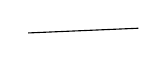
\begin{tikzpicture}
\draw (0,0) -- (1.4,0.06);
\end{tikzpicture}}

Variant of the preceding study for the extension $G_{\rho,\sigma}$ of
$\mathbb O_{12}^{*}\times H_{S_0}^{+}$ by
$\underline{M}$ (\uline{without division by}
$\underline{\mu}_G=\{1,\omega\}_{S_0}$). Let us first consider the question of the
splittings of the subextension $\underline{\mathfrak{S}}^{+}$ of
$H_{S_0}^{+}$ by $\underline{M}$ --- \unsure{they|they}
correspond to the pairs

\margin{113}
